
##########################------   END  -------#################################

\section{Code}
    \begin{frame}[plain]
        \vfill
      \centering
      \begin{beamercolorbox}[sep=8pt,center,shadow=true,rounded=true]{title}
        \usebeamerfont{title}\insertsectionhead\par%
        \color{oxfordblue}\noindent\rule{10cm}{1pt} \\
        \LARGE{\faFileCodeO}
      \end{beamercolorbox}
      \vfill
  \end{frame}

\subsection{Example}
\begin{frame}[fragile]{Example}
\begin{block}{Greatest Common Divisor}
\begin{lstlisting}[firstnumber=1, label=glabels, xleftmargin=10pt]
def greatest_c_remainder(a,b):
	'''Greatest common divisor of a and b'''
	r = a % b
	if r == 0:
		return b
	else:
		m = b
		n = r
	return greatest_c_remainder(m,n)

\end{lstlisting}
\end{block}
\end{frame}

\begin{frame}{Sobel Edge Detection %~\cite{hjelmervik2019detection}
}
\only<1>{

\vspace{-20pt}\begin{equation}
    \underline{\underline{{G}}}_{{x d}}=\left[\begin{array}{ccc}{1} & {0} & {-1} \\
                                                        					  {2} & {0} & {-2} \\
                                                       					   {1} & {0} & {-1}
                                      				  \end{array}\right]
                             						* \underline{\underline{X}}_{d}
\end{equation}

\begin{equation}
    \underline{\underline{{G}}}_{{y} d }=\left[\begin{array}{ccc}{1} & {2} & {1} \\
                                                     						{0} & {0} & {0} \\
                                                     						{-1} & {-2} & {-1}
                                            					 \end{array}\right]
                                        				* \underline{\underline{X}}_{d}
\end{equation}

Can combine these together to give a single number for the strength of the edge in
the principal component at that point:

\begin{equation}
    {G}^n_{{d}}=
    \sqrt{{{G}^n_{{x}{ d}}}^{2}
        + {{G}^n_{{y  d}}}^{2}}.
\end{equation}

To scale this the value of \(\underline{\underline{{G}}}_{{d}}\) can be expressed as some number
    of \(\sigma\) above the mean, although \({G}^n_{{d}}>0\) and not normal.}
\only<2>{
Deleting un-needed formula.
}
\end{frame}


\section{Equations}
    \begin{frame}[plain]
        \vfill
      \centering
      \begin{beamercolorbox}[sep=8pt,center,shadow=true,rounded=true]{title}
        \usebeamerfont{title}\insertsectionhead\par%
        \color{oxfordblue}\noindent\rule{10cm}{1pt} \\
        \LARGE{\faFileTextO}
      \end{beamercolorbox}
      \vfill
  \end{frame}


  { % all template changes are local to this group.
    \setbeamertemplate{navigation symbols}{}
    \begin{frame}<article:0>[plain]

        \begin{tikzpicture}[remember picture,overlay]
            \node[at=(current page.center)] {
                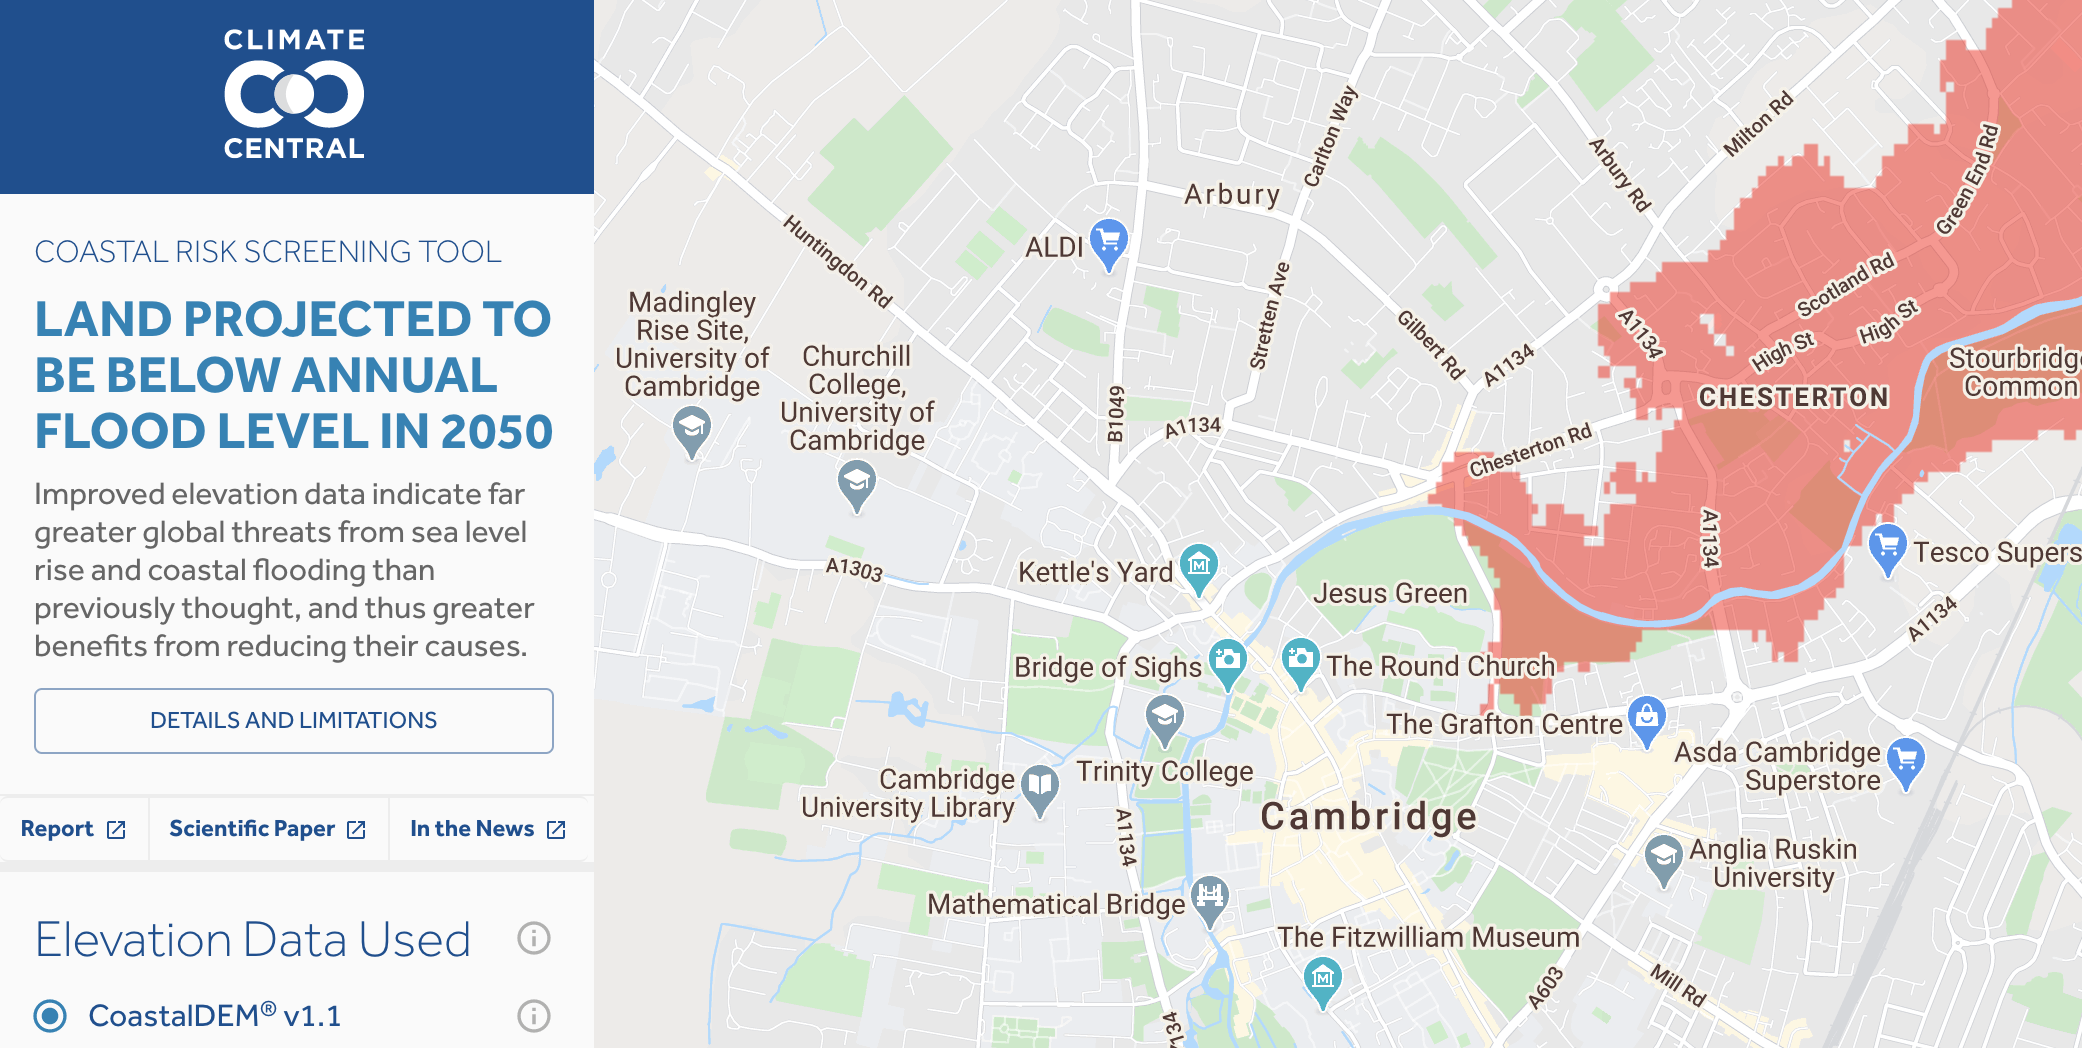
\includegraphics[keepaspectratio,
                                 width=\paperwidth,
                                 % height=\paperheight
                                 ]{example-images/cambridge-surge.png}
            };
        \end{tikzpicture}

          %\url{https://coastal.climatecentral.org/map/6/}
     \end{frame}
}

{ % all template changes are local to this group.
    \setbeamertemplate{navigation symbols}{}
    \begin{frame}<article:0>[plain]
        \begin{tikzpicture}[remember picture,overlay]
            \node[at=(current page.center)] {
                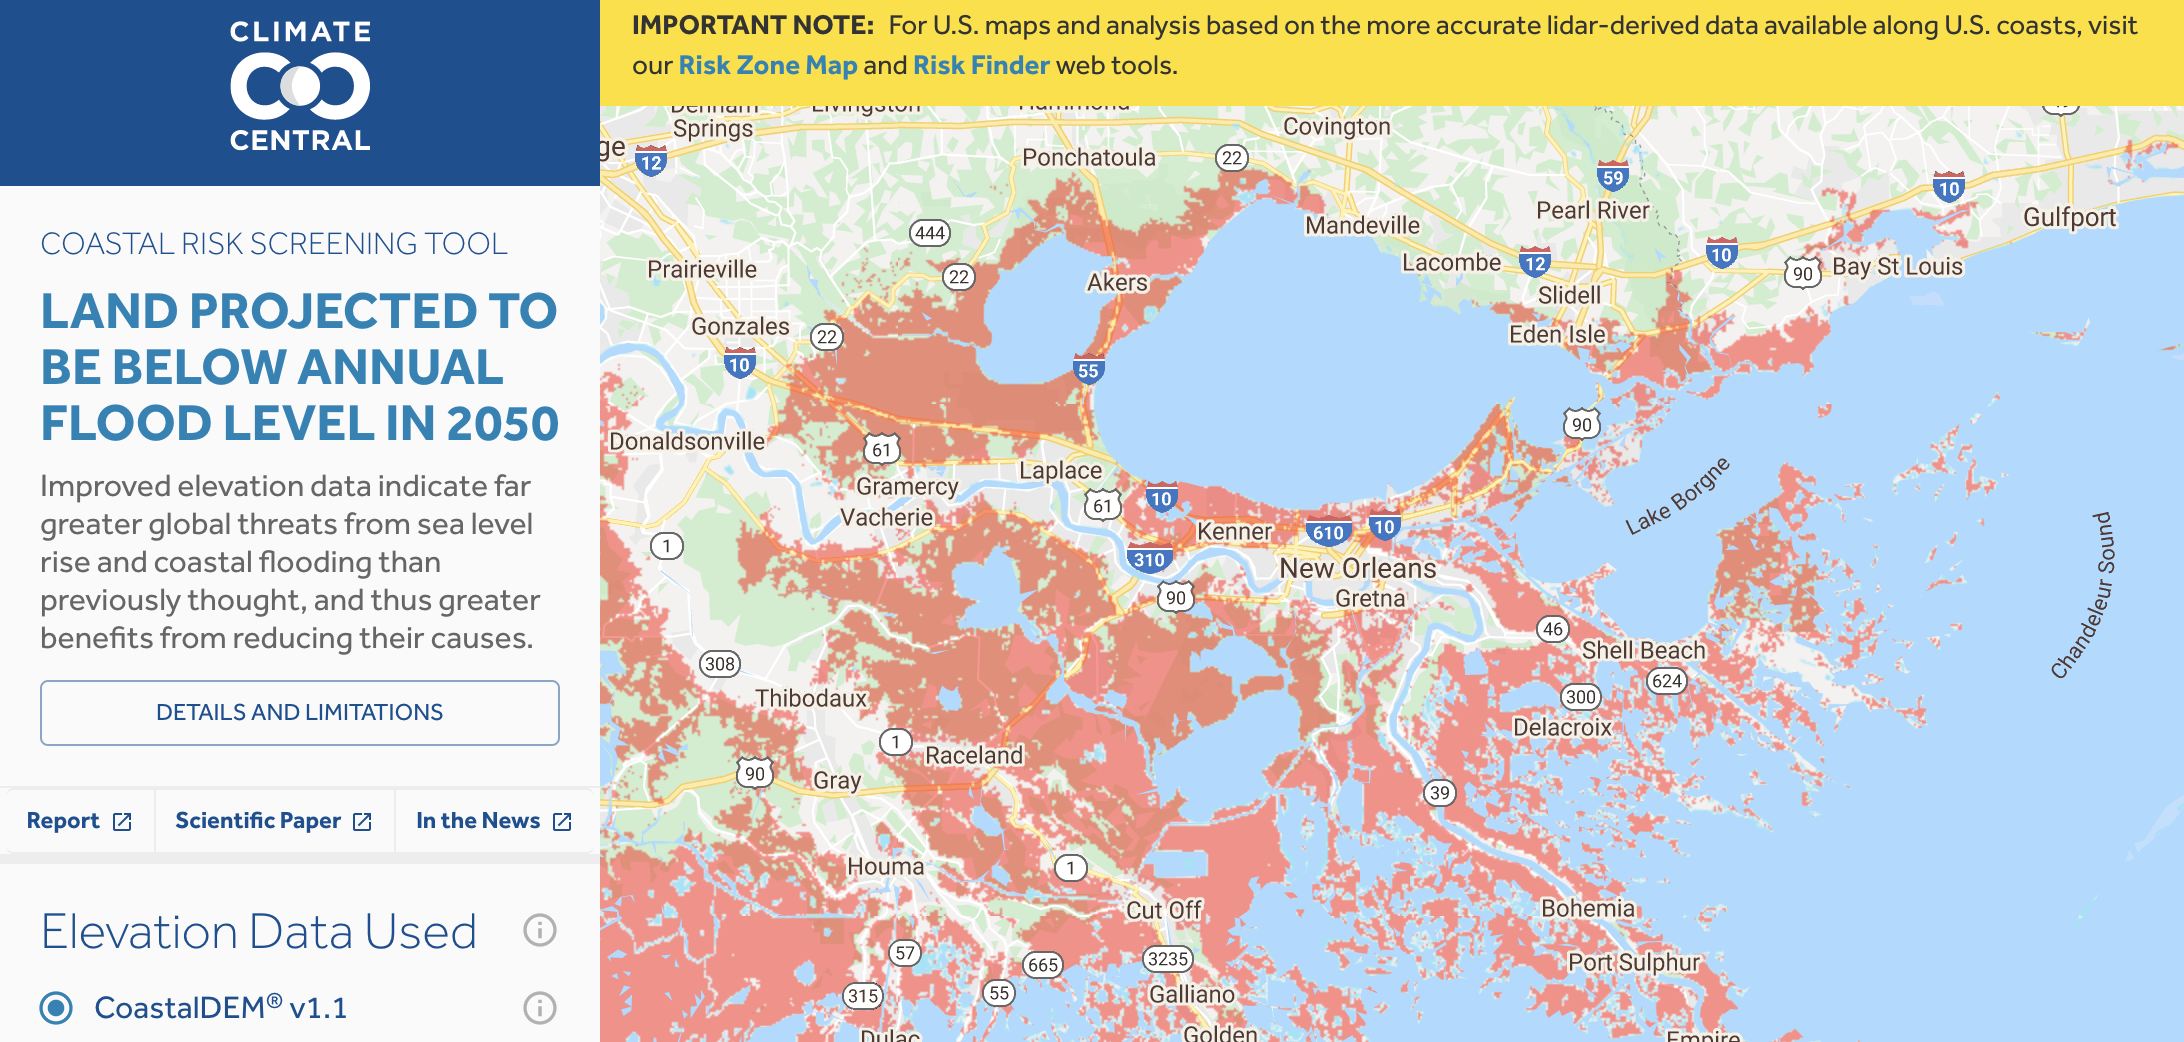
\includegraphics[keepaspectratio,
                                             width=\paperwidth,
                                            % height=\paperheight
                                            ]{example-images/new-orleans-surge.png}

            };
        \end{tikzpicture}
                  %\url{https://coastal.climatecentral.org/map/6/}
     \end{frame}
}


%\section*{Outline}\begin{frame}{Outline}\tableofcontents\end{frame}

% \section{Text}
%    \begin{frame}[plain]
%        \vfill
%      \centering
%      \begin{beamercolorbox}[sep=8pt,center,shadow=true,rounded=true]{title}
%        \usebeamerfont{title}\insertsectionhead\par%
%        \color{oxfordblue}\noindent\rule{10cm}{1pt} \\
%        \LARGE{\faFileTextO}
%      \end{beamercolorbox}
%      \vfill
%  \end{frame}
